\subsection{Bernstein-Bézier Splines (B-B-Splines)}
The bernstein-Bézier splines should give the same result as the cubic splines mentioned in the previous chapter. The difference is that one does not get a single formula in the end, but different data points. A good explanation can be found in the following \href{https://youtu.be/aVwxzDHniEw}{video}. But first of all to understand bézier curves/spline one must be familiar with Bernstein polynomials and therefore with the binomial coefficient (see also \autoref{eq:binomial_coefficient})
\begin{equation}\label{eq:binomial_coefficient}
\left(\begin{array}{l}
n \\
k
\end{array}\right)=\frac{n !}{k !(n-k) !}
\end{equation}
\begin{figure}[ht]
  \centering
  \resizebox{0.7\textwidth}{!}{\subimport{images/}{pascals_triangle}}
  \caption{Pascal's triangle formula}
  \label{fig:pascals_triangle}
\end{figure}
\begin{figure}[ht]
  \centering
  \resizebox{0.7\textwidth}{!}{\subimport{images/}{pascals_triangle_2}}
  \caption{Pascal's triangle numbers}
  \label{fig:pascals_triangle_2}
\end{figure}\newline
\paragraph{Example: (For what can the binomial coefficients be used?)}
What is the \textcolor{blue}{fourth} term of $(3x-4y)^{\textcolor{red}{6}}$ (note there is no zeroth term, therefore we subtract \textcolor{brown}{one} in the equation blew)? The result can also be read from \autoref{fig:pascals_triangle_2}.
$$
\left(\begin{array}{l}
\textcolor{red}{6} \\
\textcolor{blue}{4}-\textcolor{brown}{1}
\end{array}\right)=\frac{\textcolor{red}{6} !}{(\textcolor{blue}{4}-1) !(\textcolor{red}{6}-(\textcolor{blue}{4}-1)) !} = 20
$$
Therefore, the fourth term is:
$$
20 \cdot \left( (3x)^{\textcolor{red}{6}-(\textcolor{blue}{4}-1)}\cdot(-4y)^{(\textcolor{blue}{4}-1)}\right)=20 \cdot \left(27 \cdot x^3 \cdot (-64)y^4\right)=-34560x^2y^4
$$
This is much easier than to really calculate the polynomial. An explanation can also be found in the following \href{https://youtu.be/s19dWIHficY}{video}



\subsubsection{Bernstein Polynomial}
The bernstein polynomial is defined in \autoref{eq:bernstein_polynomial}.
\begin{equation}\label{eq:bernstein_polynomial}
B_{\text {i\textcolor{ForestGreen}{n} }}(t)=\left(\begin{array}{c}
\textcolor{ForestGreen}{n} \\
i
\end{array}\right)(1-t)^{\textcolor{ForestGreen}{n}-i} t^i \quad t \in[0,1] \quad(i=0,1, \cdots, \textcolor{ForestGreen}{n})
\end{equation}


In \autoref{eq:bernstein_polynomial} one had an interval $\in[0, 1]$. When our data is in another range like $\in[a, b]$ one has to use \autoref{eq:bernstein_polynomial_transformed}
\begin{equation}\label{eq:bernstein_polynomial_transformed}
\resizebox{1\textwidth}{!}{$
B_{i \textcolor{ForestGreen}{n}}(u, a, b)=B_{\text {i\textcolor{ForestGreen}{n} }}\left(\frac{u-a}{b-a}\right)=\frac{1}{(b-a)^{\textcolor{ForestGreen}{n}}}\left(\begin{array}{l}
\textcolor{ForestGreen}{n} \\
i
\end{array}\right)(b-u)^{n-i}(u-a)^i \quad u \in[a, b] \quad(i=0,1, \cdots, \textcolor{ForestGreen}{n})$}
\end{equation}
Furthermore note that those polynomials look like one can see in \autoref{fig:bernstein_poly}. 
\begin{figure}[ht!]
    \centering
    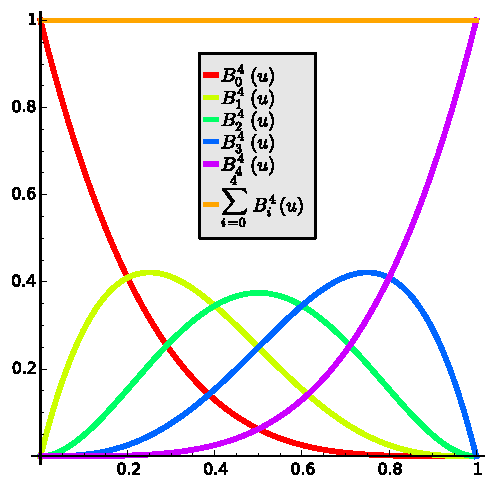
\includegraphics[width=0.6\textwidth]{images/bernstein_poly.pdf}
    \caption{Plot of Bernstein polynomial functions up to degree 4 with summation of all four functions to show characteristic of partition of one (Note the maximum of each polynomial is always at $t=\frac{i}{\textcolor{ForestGreen}{n}}$)}
    \label{fig:bernstein_poly}
\end{figure}
The polynomials relate to each other, as one can see in \autoref{eq:bernstein_polynomial_relation}.
\begin{equation}\label{eq:bernstein_polynomial_relation}
\begin{aligned}
& \frac{d}{d t} B_{i, n}(t)=n\left(B_{i-1, n-1}(t)-B_{i, n-1}(t)\right)=-n \Delta B_{i-1, n-1}(t) \\
& \frac{d^{2}}{d t^{2}} B_{i, n}(t)=n(n-1)\left(B_{i-2, n-2}(t)-2 B_{i-1, n-2}(t)+B_{i, n-2}(t)\right)=n(n-1) \Delta^{2} B_{i-2, n-2}(t) \\
& \frac{d^{k}}{d t^{k}} B_{i, n}(t)=(-1)^{k} n(n-1) \ldots(n-k+1) \Delta^{k} B_{i-k, n-k}(t)
\end{aligned}
\end{equation}
\FloatBarrier
\subsubsection{Simple Bézier Curves}
A \textcolor{Plum}{simple Bézier curve} is defined with \autoref{eq:simple_bezier_curve}. To get the idea also have a look at \autoref{fig:bezier_curve}.
\begin{equation}\label{eq:simple_bezier_curve}
\textcolor{Plum}{\vec{r}(t)}=\sum_{\textcolor{green}{i}=0}^{\textcolor{ForestGreen}{n}} \vec{P}_{\textcolor{green}{i}} B_{\textcolor{green}{i} \textcolor{ForestGreen}{n}}(t) \quad t \in[0,1]
\end{equation}
Where:
\begin{itemize}
    \item $\textcolor{green}{i}$ control point number
    \item $\textcolor{ForestGreen}{n}$ is the total number of control points minus one, since Points are ($P_0, P_1, P_2, P_n$)
\end{itemize}
\subsubsection{Composite Bézier Curves}
The simple Bézier curves meet at common control points. Which is a continuity condition ($C^0$), but often higher (smoothness) conditions are required ($C^k$-smooth). This condition is only met if and only if \autoref{eq:bezier_smooth_condition} is given.
\begin{equation} \label{eq:bezier_smooth_condition}
\frac{\Delta^{\ell} \vec{P}_{\textcolor{ForestGreen}{n}-\ell, j}}{h_j^{\ell}}=\frac{\Delta^{\ell} \vec{P}_{0, j+1}}{h_{j+1}^{\ell}} \quad(j=0,1, \cdots, m-2 \quad \ell=0,1,2, \cdots, k)
\end{equation}
Writing out \autoref{eq:bezier_smooth_condition} for $C^1$ smoothness results in \autoref{eq:bezier_smooth1}, whereas $C^2$ smoothness results in  \autoref{eq:bezier_smooth2} where one has to know that also \autoref{eq:bezier_smooth1} $C^1$ smoothness must be met.
\begin{equation}\label{eq:bezier_smooth1}
\frac{\textcolor{ForestGreen}{n}\left(\vec{P}_{\textcolor{ForestGreen}{n}, \textcolor{orange}{j}}-\vec{P}_{\textcolor{ForestGreen}{n}-1, \textcolor{orange}{j}}\right)}{h_{\textcolor{orange}{j}}}=\frac{\textcolor{ForestGreen}{n}\left(\vec{P}_{1, \textcolor{orange}{j}+1}-\vec{P}_{0, \textcolor{orange}{j}+1}\right)}{h_{\textcolor{orange}{j}+1}} \quad(\textcolor{orange}{j}=0,1, \cdots, m-2)
\end{equation}
\begin{equation}\label{eq:bezier_smooth2}
\frac{\textcolor{ForestGreen}{n}(\textcolor{ForestGreen}{n}-1)\left(\vec{P}_{\textcolor{ForestGreen}{n}, \textcolor{orange}{j}}-2 \vec{P}_{\textcolor{ForestGreen}{n}-1, \textcolor{orange}{j}}+\vec{P}_{\textcolor{ForestGreen}{n}-2, \textcolor{orange}{j}}\right)}{h_{\textcolor{orange}{j}}{ }^2}=\frac{\textcolor{ForestGreen}{n}(\textcolor{ForestGreen}{n}-1)\left(\vec{P}_{2, \textcolor{orange}{j}+1}-2 \vec{P}_{1, \textcolor{orange}{j}+1}+\vec{P}_{0, \textcolor{orange}{j}+1}\right)}{h_{\textcolor{orange}{j}+1}{ }^2} \quad(\textcolor{orange}{j}=0,1, \cdots, m-2)
\end{equation}

The Bézier-curve is defined by the control points $\left(\vec{P}_{\textcolor{green}{0}}, \vec{P}_{\textcolor{green}{1}}, \ldots \vec{P}_{\textcolor{green}{n}}(\textcolor{ForestGreen}{n} \geq 2)\right)$ and the  Bernstein polynomials. On each \textcolor{orange}{spline} one has \textcolor{ForestGreen}{n}+1 \textcolor{green}{control points}.
\begin{itemize}
    \item \textcolor{orange}{spline number}, the spline number there are m splines (m=(Number of given Data points-1))
    \item \textcolor{green}{point on spline}, there are $\textcolor{ForestGreen}{n}+1$ points on the spline
\end{itemize}
$$
\vec{r}_{\textcolor{orange}{j}}(u)=\sum_{\textcolor{green}{i}=0}^{\textcolor{ForestGreen}{n}} \vec{P}_{\textcolor{green}{i}, \textcolor{orange}{j}} B_{\textcolor{green}{i} \textcolor{ForestGreen}{n}}\left(u, u_j \cdot u_{j+1}\right) \quad u \in\left[u_j \cdot u_{j+1}\right] \quad(j=0,1, \cdots, m-1)
$$
\begin{figure}[ht!]
    \centering
    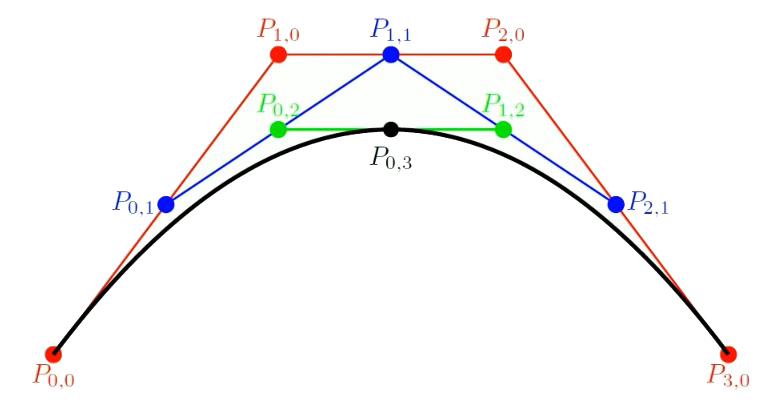
\includegraphics[width=0.8\textwidth]{images/cubic_bezier_curve.jpg}
    \caption{Cubic Bézier Curve (Always defined by 4 control points), degree three}
    \label{fig:bezier_curve}
\end{figure}
\subsubsection{Example: Composite Bézier Curves}
The four points $A=(0,0), B=(1,0), C=(2,3)$ and $D=(2,4)$ are to be interpolated (joined) by composed $C^1$ Bernstein-Bézier splines: $A$ and $B$ are to be joined  linearly (by a straight line), as well as $C$ and $D$.\newline Compute the missing $C^1$ Bernstein-Bézier spline of minimal degree between $B$ and $C$. \newline\newline
To solve the exercise one can use \autoref{eq:bezier_smooth1}. Where the first \textcolor{orange}{spline} and the last one have two control points, since it is a straight line $\Rightarrow$ $\textcolor{ForestGreen}{n}=\textcolor{violet}{1}$. The second \textcolor{orange}{spline} has four conditions, since tow points must be met and two derivatives, since it must be $C^1$ smooth. Due to that $\textcolor{ForestGreen}{n}=\textcolor{pink}{3} \Rightarrow$ the degree is also 3 (also called cubic).
$$
\begin{aligned}
    &\textcolor{violet}{1} \cdot \left(P_{\textcolor{green}{1}, \textcolor{orange}{0}}-P_{\textcolor{green}{0}, \textcolor{orange}{0}}\right)=\textcolor{pink}{3} \cdot \left(P_{\textcolor{green}{1}, \textcolor{orange}{1}}-P_{\textcolor{green}{0}, \textcolor{orange}{1}}\right)=\textcolor{violet}{1}\cdot \left(\left(\begin{array}{l} 1 \\ 0 \end{array}\right)-\left(\begin{array}{l} 0 \\ 0 \end{array}\right)\right)=\textcolor{pink}{3}\cdot\left(P_{\textcolor{green}{1}, \textcolor{orange}{1}}-\left(\begin{array}{l} 1 \\ 0 \end{array}\right)\right)\\
    & \textcolor{pink}{3} \cdot \left(P_{\textcolor{green}{3}, \textcolor{orange}{1}}-P_{\textcolor{green}{2}, \textcolor{orange}{1}}\right)=\textcolor{violet}{1}\cdot\left(P_{\textcolor{green}{1}, \textcolor{orange}{2}}-P_{\textcolor{green}{0}, \textcolor{orange}{2}}\right)=\textcolor{pink}{3}\cdot \left(\left(\begin{array}{l} 2 \\ 3 \end{array}\right)-P_{\textcolor{green}{2}, \textcolor{orange}{1}}\right)=\textcolor{violet}{1}\cdot\left(\left(\begin{array}{l} 0 \\ 0 \end{array}\right)-\left(\begin{array}{l} 1 \\ 0 \end{array}\right)\right)\\
    &\Rightarrow P_{\textcolor{green}{1}, \textcolor{orange}{1}}=\left(\begin{array}{l} \frac{4}{3} \\ 0 \end{array}\right)\\
    &\Rightarrow P_{\textcolor{green}{2}, \textcolor{orange}{1}}=\left(\begin{array}{l} 2 \\ \frac{8}{3} \end{array}\right)
\end{aligned}
$$
$$
\begin{aligned}
\vec{r}(t) & =\underbrace{P_{\textcolor{green}{0}, \textcolor{orange}{1}}}_B \cdot B_{03}(t)+P_{\textcolor{green}{1}, \textcolor{orange}{1}} \cdot B_{13}(t)+P_{\textcolor{green}{2}, \textcolor{orange}{1}} \cdot B_{23}(A)+\underbrace{P_{\textcolor{green}{0}, \textcolor{orange}{1}}}_C \cdot B_{33} \\
& =\left(\begin{array}{l}
1 \\
0
\end{array}\right)(1-t)^3+3\left(\begin{array}{l} \frac{4}{3} \\ 0 \end{array}\right)(1-t)^2 t+3\left(\begin{array}{l}
2 \\
\frac{8}{3}
\end{array}\right)(1-t) t^2+\left(\begin{array}{l}
2 \\
3
\end{array}\right) t^3
\end{aligned}
$$
$$
t \in[0,1]
$$
% \begin{wrapfigure}{R}{0.5\textwidth}
\begin{figure}[ht]
  \centering
  \resizebox{0.5\textwidth}{!}{\subimport{images/}{bezier}}
  \caption{Exercise Overview}
  \label{fig:bezier}
\end{figure}
\FloatBarrier

\subsubsection{Properties}
\begin{itemize}
    \item The Bézier-curves is always inside the convex hull of the data points.
    \item$$
    \begin{aligned}
    & \vec{r}(0)=\vec{P}_{0} \quad \vec{r}(1)=\vec{P}_{n} \\
    & \vec{r}^{\prime}(0)=n\left(\vec{P}_{1}-\vec{P}_{0}\right) \quad \vec{r}^{\prime}(1)=n\left(\vec{P}_{n}-\vec{P}_{n-1}\right) \\
    & \vec{r}^{\prime \prime}(0)=n(n-1)\left(\vec{P}_{2}-2 \vec{P}_{1}+\vec{P}_{0}\right) \quad \vec{r}^{\prime \prime}(1)=n(n-1)\left(\vec{P}_{n}-2 \vec{P}_{n-1}+\vec{P}_{n-2}\right)
    \end{aligned}
    $$
    \item If $C^{k}$ smoothness for a point is required, $k$ equations or $k$ control points are necessary
\end{itemize}
\subsubsection{Casteljau recurrence}
The Casteljau recurrence is a similar idea as the neville-aitken. With this Idea a point on the Bézier curve can be calculated as a linear combination of two points on a Bézier curve of a lower degree.
$$
\vec{r}_{\overrightarrow{P_{0}}, \overrightarrow{P_{1}}, \ldots, \overrightarrow{P_{n}}}(t)=(1-t) \cdot \vec{r}_{\overrightarrow{P_{0}}, \overrightarrow{P_{1}}, \ldots, P_{n-1}} \overrightarrow{ }(t)+t \cdot \vec{r}_{\overrightarrow{P_{1}}, \overrightarrow{P_{2}}, \ldots, \overrightarrow{P_{n}}}(t) \quad t \in[0,1]
$$

$$
\begin{array}{llll}
C^{0}: & &  P_{n}=\vec{Q}_{0} \\
C^{1}: & \vec{r}_{P}^{\prime}(1)= & n\left(\vec{P}_{n}-\vec{P}_{n-1}\right)=m\left(\vec{Q}_{1}-\vec{Q}_{0}\right) & =\vec{r}_{Q}^{\prime}(0) \\
C^{2}: & \vec{r}_{P}^{\prime \prime}(1)= & n(n-1)\left(\vec{P}_{n}-2 \vec{P}_{n-1}+\vec{P}_{n-2}\right)=m(m-1)\left(\vec{Q}_{2}-2 \vec{Q}_{1}+\vec{Q}_{0}\right) & =\vec{r}_{Q}^{\prime \prime}(0) \\
C^{k}: & \vec{r}_{P}^{(k)}(1)= & n(n-1) \ldots(n-k+1)\left(\Delta^{k} \vec{P}_{n-k}\right)=m(m-1) \ldots(m-k+1)\left(\Delta^{k} \vec{Q}_{0}\right) & =\vec{r}_{Q}^{(k)}(0)
\end{array}
$$
Is $\overrightarrow{r_{j}}(t)=\sum_{i=0}^{n} \vec{P}_{i, j} B_{i, n}(t) \quad t \in[0,1]$ with the functions $Q_{j}$ defined (degree: $n$ ), the following formulas turn out:
$$
\begin{array}{llll}
C^{0}: & \vec{P}_{n, j-1}=\vec{P}_{0, j}=\vec{Q}_{j} \\
C^{1}: & \vec{r}_{j-1}^{\prime}(1)= & \vec{Q}_{j}-\vec{P}_{n-1, j-1}=\vec{P}_{1, j}-\vec{Q}_{j} & =\vec{r}_{j}^{\prime}(0) \\
C^{2}: & \vec{r}_{j-1}^{\prime \prime}(1)= & \vec{Q}_{j}-2 \vec{P}_{n-1, j-1}+\vec{P}_{n-2, j-1}=\vec{P}_{2, j}-2 \vec{P}_{1, j}+\vec{Q}_{j} & =\vec{r}_{j}^{\prime \prime}(0) \\
C^{k}: & \vec{r}_{j-1}^{(k)}(1)= & \Delta^{k} \vec{P}_{n-k, j-1}=\Delta^{k} \vec{P}_{0, j} & =\vec{r}_{j}^{(k)}(0)
\end{array}
$$





\subsubsection{Example}
Let's do the same example as in \autoref{subsubsec:ex_spline}. Where the following four points are given: 
$$\left\{\underbrace{(0,0)}_{Q_0=P_{\textcolor{green}{0}, \textcolor{orange}{0}}},\underbrace{\left(\frac{\pi}{3}, \frac{\sqrt{3}}{2}\right)}_{Q_1=P_{\textcolor{green}{0}, \textcolor{orange}{1}}=P_{\textcolor{green}{3}, \textcolor{orange}{0}}},\left(\frac{2 \pi}{3}, \frac{\sqrt{3}}{2}\right),(\pi, 0)\right\}$$
Therefore $\vec{Q}_0=(0,0), \vec{Q}_1=\left(\frac{\pi}{3}, \frac{\sqrt{3}}{2}\right), \dots$ and $h_j=h=\frac{\pi}{3}$. One now has to met the following requirements: 

$$
\begin{aligned}
&\vec{Q}_1-\vec{P}_{\textcolor{green}{2},\textcolor{orange}{0}}=\vec{P}_{\textcolor{green}{1},\textcolor{orange}{1}}-\vec{Q}_1 \\
&\vec{Q}_2-\vec{P}_{2,1}=\vec{P}_{1,2}-\vec{Q}_2 \\
&\vec{Q}_1-2 \vec{P}_{2,0}+\vec{P}_{1,0}=\vec{P}_{2,1}-2 \vec{P}_{1,1}+\vec{Q}_1 \\
&\vec{Q}_2-2 \vec{P}_{2,1}+\vec{P}_{1,1}=\vec{P}_{2,2}-2 \vec{P}_{1,2}+\vec{Q}_2
\end{aligned}
$$

$$
\begin{aligned}
&\vec{P}_{2,0}-2 \vec{P}_{1,0}+\vec{Q}_0=\overrightarrow{0} \\
&\vec{Q}_3-2 \vec{P}_{2,2}+\vec{P}_{1,2}=\overrightarrow{0}
\end{aligned}
$$

The solution of the linear system above gives us the following points:
$$
\left\{\underbrace{\left\{\frac{\pi}{9}, \frac{\sqrt{3}}{5}\right\}}_{P_{\textcolor{green}{1}, \textcolor{orange}{0}}},\underbrace{\left\{\frac{2 \pi}{9}, \frac{2 \sqrt{3}}{5}\right\}}_{P_{\textcolor{green}{2}, \textcolor{orange}{0}}},\underbrace{\left\{\frac{4 \pi}{9}, \frac{3 \sqrt{3}}{5}\right\}}_{P_{\textcolor{green}{1}, \textcolor{orange}{1}}},\underbrace{\left\{\frac{5 \pi}{9}, \frac{3 \sqrt{3}}{5}\right\}}_{P_{\textcolor{green}{2}, \textcolor{orange}{1}}},\left\{\frac{7 \pi}{9}, \frac{2 \sqrt{3}}{5}\right\},\left\{\frac{8 \pi}{9}, \frac{\sqrt{3}}{5}\right\}\right\}
$$

When we now calculate the first spline we get the same result as before.
\begin{equation}
\begin{aligned}
\vec{r_1}(t)&=\left(\begin{array}{c}
\frac{1}{9} \pi \mathrm{B}_{1,3}(t)+\frac{2}{9} \pi \mathrm{B}_{2,3}(t)+\frac{1}{3} \pi \mathrm{B}_{3,3}(t) \\
\frac{1}{5} \sqrt{3} \mathrm{~B}_{1,3}(t)+\frac{2}{5} \sqrt{3} \mathrm{~B}_{2,3}(t)+\frac{1}{2} \sqrt{3} \mathrm{~B}_{3,3}(t)
\end{array}\right)\\
&=\left(\begin{array}{l}
\frac{\pi}{9} 3(1-t)^2 t+\frac{2 \pi}{9} 3(1-t) t^2+\frac{1}{3} \pi t^3 \\
\frac{\sqrt{3}}{5} 3(1-t)^2 t+\frac{2}{5} \sqrt{3} 3(1-t) t^2+\frac{\sqrt{3}}{2} t^3
\end{array}\right)\\
&=\left(\begin{array}{l}
x \\
y
\end{array}\right)\\
\Longleftrightarrow & \left(\begin{array}{c}
\frac{\pi}{3} t=x \\
\frac{3 \sqrt{3}}{5} t-\frac{\sqrt{3}}{10} t^3=y
\end{array}\right) \Rightarrow\left(\begin{array}{l}
t=\frac{3 x}{\pi} \\
y=\frac{9 \sqrt{3}}{5 \pi} x-\frac{27 \sqrt{3}}{10 \pi^3} x
\end{array}\right)
\end{aligned}
\end{equation}
For the second spline we get the following:
\begin{equation}
\left(\begin{array}{c}
\frac{1}{3} \pi \mathrm{B}_{0,3}(t)+\frac{4}{9} \pi \mathrm{B}_{1,3}(t)+\frac{5}{9} \pi \mathrm{B}_{2,3}(t)+\frac{2}{3} \pi \mathrm{B}_{3,3}(t) \\
\frac{1}{2} \sqrt{3} \mathrm{~B}_{0,3}(t)+\frac{3}{5} \sqrt{3} \mathrm{~B}_{1,3}(t)+\frac{3}{5} \sqrt{3} \mathrm{~B}_{2,3}(t)+\frac{1}{2} \sqrt{3} \mathrm{~B}_{3,3}(t)
\end{array}\right)
\end{equation}
